\documentclass[a4paper, 12pt]{article}

\usepackage{geometry}

\usepackage[utf8]{inputenc}
\usepackage[italian]{babel}
\usepackage[T1]{fontenc}
\usepackage{listings}
\usepackage[numbered, framed]{matlab-prettifier}
\usepackage{hyperref}
\usepackage{amsmath}
\usepackage{graphicx}

\usepackage{subcaption}
\usepackage{algorithm}
\usepackage{algorithmic}
\renewcommand{\algorithmicrequire}{\textbf{Input:}}
\renewcommand{\algorithmicensure}{\textbf{Output:}}

\graphicspath{{./images/}}

% Title Page.
\title{\textbf{\Huge Metodi Numerici\\ per la Grafica\\ \vspace{1cm}- Relazione -\\ \vspace{1cm} Superfici di Bezier e B-Spline}}
\author{Marco Calamai - Elia Mercatanti}

\begin{document}
	
\begin{titlepage}
	\maketitle
\end{titlepage}

\tableofcontents
\lstlistoflistings
\listoffigures

\newpage

\section{Base delle B-spline}

Sia assegnato $I = [\tau_0, \tau_L]$ e dato un vettore esteso di nodi
$$ \mathbf{t} =  \left\{ \underbrace{t_{0}, \dots, t_{k-2}}_{k-1}, \underbrace{t_{k-1}, \dots, t_{n+1}}_{\tau_0, \tau_1, \dots, \tau_1 \dots, \tau_{L-1}, \dots, \tau_{L-1} ,\tau_L}, \underbrace{t_{n+2}, \dots, t_{n+k}}_{k-1} \right\} $$
con
$$t_0 \leq t_1 \leq \dots t_{k+1} \leq  t_k \dots \leq  t_{n+1} \leq t_{n+2} \leq \dots \leq t_{n+k}$$
in cui ogni nodo $\tau_i$ è ripetuto con molteplicità $m_i$ , $i = 1, \dots , L-1$.\\
Possiamo definire la base delle B-spline come l'insieme delle funzioni B-spline definite sul vettore esteso di nodi dalla formula ricorrente di \textit{Cox - De Boor}
$$N_{i, r}(t) = \omega_{i,r}(t)N_{i, r-1}(t) + [1-\omega_{i+1, r}(t)]N_{i+1, r-1}$$
con
$$\omega_{i,r}(t) = \begin{cases} \frac{t-t_i}{t_{i+r-1}-t_i}, & \text{se } t<t_{i+r-1} \\ 0, & \text{altrimenti} \end{cases}$$
dove
$$N_{i, 1}(t) = \begin{cases} 1, & \text{se } t\in[t_i, t_{i+1}] i = 0, \dots, n+k-1 \\ 0, & \text{altrimenti} \end{cases}$$
Nel seguente codice Matlab \ref{code:coxdeboor}  sono state implementate le funzioni descritte sopra per il calcolo delle basi di \textit{Cox - De Boor}.\\
La funzione principale è \texttt{cox\_deBoor}, la quale si occupa di calcolare le basi delle B-Spline richiamando la funzione \texttt{omega} per il calcolo dei coefficienti $\omega_{i,r}$ nella relazione ricorrente di \textit{Cox - De Boor}.\\
A livello implementativo, nella funzione \texttt{cox\_deBoor} la parte più delicata è il controllo da effettuare nel caso in cui l'ordine della B-Spline sia $1$. In quel caso la funzione restituisce $1$ se il valore di $t\_star$ cade nell'intervallo $[t_i, t_{i+1}) $ ma nel caso in cui si trovasse nell'ultimo intervallo, bisogna prendere in considerazione anche l'ultimo valore dell'intervallo.\\
Per quanto riguarda invece la funzione \texttt{omega}, è stato previsto un controllo per fare in modo che restituisca zero nel caso di denominatore nullo, che si può verificare in caso di nodi con molteplicità maggiore di uno.

\lstinputlisting[label=code:coxdeboor, style=Matlab-editor, caption=B-Spline tramite relazione ricorrente di Cox - de Boor, basicstyle=\footnotesize\ttfamily]{../cox_de_boor.m}

Per disegnare degli esempi di basi B-Spline abbiamo utilizzato lo sript \ref{code:BasiBSpline} in cui viene richiamata la funzione \ref{code:coxdeboor} per il calcolo delle basi di \textit{Cox - De Boor} vista prima.\\
In figura \ref{fig:BernsteinBaseExample} sono riportate le sei funzioni di un'esempio di base di Bernstein di ordine 6, la quale rappresenta un caso particolare di B-Spline in cui, il vettore esteso dei nodi è formato solamente da $\tau_0$ ripetuto ordine volte, seguito da $\tau_L$ ripetuto ordine volte.\\
La figura \ref{fig:BSplineinBaseExample} invece mostra un esempio di base B-SPline di ordine 4 ($k = 4$) con vettore esteso di nodi definito come $t = [1, 1, 2, 3, 4, 5, 6, 6]$.

\lstinputlisting[label=code:BasiBSpline, style=Matlab-editor, caption=Disegno basi B-Spline, basicstyle=\footnotesize\ttfamily]{../b_spline_base.m}

\begin{figure}[!]
	\centering
	\caption{Esempio di base con t = [0, 0, 0, 0, 0, 0, 1, 1, 1, 1, 1, 1] e k=6}
	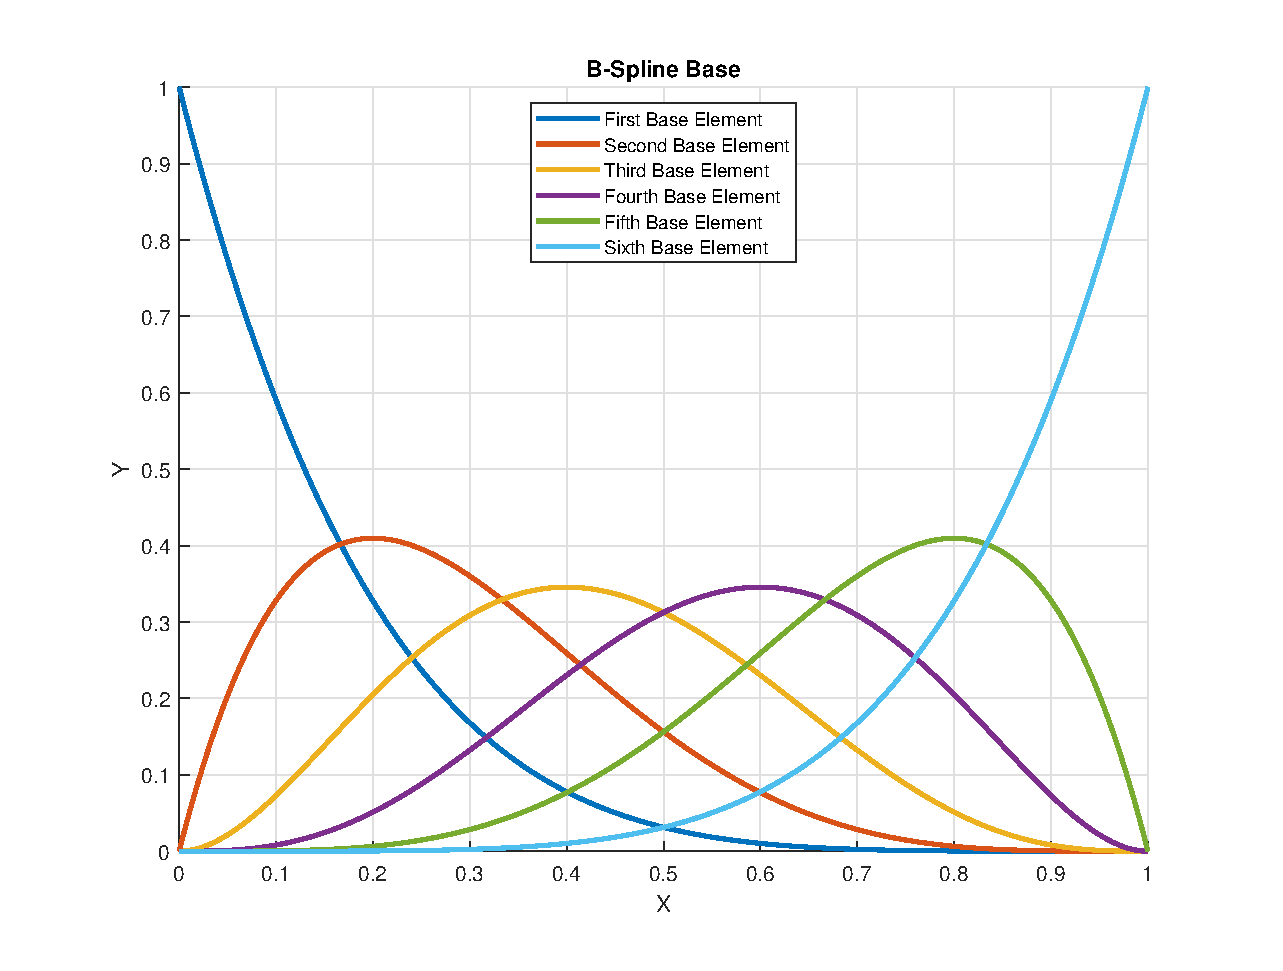
\includegraphics[scale=0.55]{plot_bezier_base.eps}
	\label{fig:BernsteinBaseExample}
\end{figure}

\begin{figure}[!]
	\centering
	\caption{Esempio di base con t = [1, 1, 2, 3, 4, 5, 6, 6] e k= 4}
	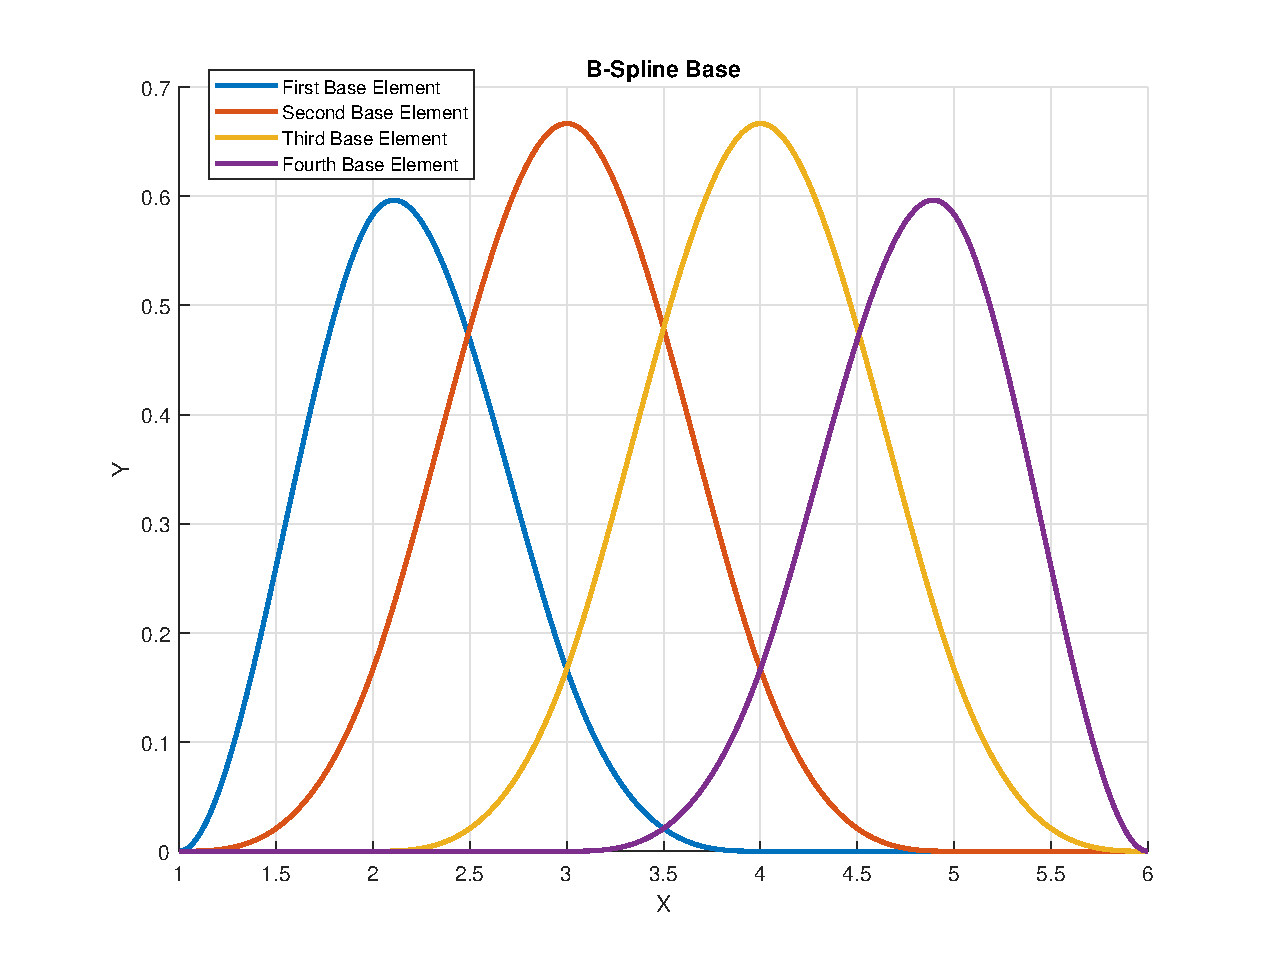
\includegraphics[scale=0.55]{plot_b-spline_base.eps}
	\label{fig:BSplineinBaseExample}
\end{figure}

\section{Le Curve B-spline}
Dati $n+1$ punti di controllo, un curva B-Spline $\mathbf{X} : [a,b] = [\tau_0, \tau_L]$ di ordine $k$ è definita a partire dalla base delle B-Spline come

$$\mathbf{X}(t) := \sum_{i=0}^{n} \mathbf{d_i} N_{i, k}(t)$$

Le curve B-Spline presenti in questa relazione sono state calcolate e rappresentate  utilizzando l'algoritmo di De Boor.\\ 
L'algoritmo di De Boor è una generalizzazione dell'algoritmo di De Casteljeau; un modo veloce e numericamente stabile per trovare un punto in una B-Spline dato un $\mathbf{u}$ appartenente al dominio. Tale algoritmo si basa sul fatto che aumentando la molteplicità di un knot interno, decresce il numero di funzioni base non nulle che attraversano questo knot, infatti, se la molteplicità di questo knot è $m$, ci sono al più $degree – m +1$ funzioni base non nulle che attraversano questo knot. Questo implica che in un nodo di molteplicità pari al grado della curva, ci sarà solo un funzione base (essendo $degree – degree + 1 = 1$ ) non nulla il cui valore in corrispondenza di tale knot sarà uguale ad $1$ per il principio della partizione dell'unità.\\
Quindi, nell'algoritmo di De Boor, un nodo $u$ viene inserito ripetutamente in modo che la sua molteplicità sia pari al grado della curva. L'ultimo nuovo punto di controllo generato sarà quindi il punto della curva che corrisponde ad $u$.\\
Nella funzione Matlab  \ref{code:De_Boor_Algorithm} è stato implementato l'algoritmo di De Boor per il calcolo e la rappresentazione di curve B-Spline. La descrizione dell'algoritmo è illustrata nello pseudo codice \ref{alg:DeBoor}.


\begin{algorithm}
	\caption{Algoritmo di De Boor}
	\begin{algorithmic} 
		\REQUIRE $\mathbf{u}$
		\ENSURE $\mathbf{C(u)}$, il valore della curva in $\mathbf{u}$.
		\IF{$\mathbf{u}$ non è un nodo già esistente}
		\STATE $h = degree$ (inseriamo $\mathbf{u}$ esattamente grado volte)
		\STATE $s = 0$
		\ELSE
		\STATE $h = degree - s$ (inseriamo $\mathbf{u}$ $degree - s$ volte, dove $s$ è la molteplicità del nodo già esistente  )
		\ENDIF
		\STATE Supponiamo che il nodo $\mathbf{u}$ si trovi nel knot span $[\mathbf{u}_l, \mathbf{u}_{l+1}$).
		\STATE Copiamo i punti di controllo che saranno influenzati dall'algoritmo $\mathbf{P}_{l-s}, \mathbf{P}_{l-s-1}, \mathbf{P}_{l-s-2}, \dots , \mathbf{P}_{l-degree+1}, \mathbf{P}_{l-degree}$ in un nuovo array e li rinominiamo come: $\mathbf{P}_{l-s,0} , \mathbf{P}_{l-s-1,0} , \mathbf{P}_{l-s-2,0} , ... , \mathbf{P}_{l-degree+1,0} , \mathbf{P}_{l-degree,0}$ dove lo 0 indica lo step iniziale (che ovviamente crescerà ad ogni passo dell'algoritmo);
		\FOR{${r}$ from $1$ to $h$} 
		\STATE {text
			\FOR {$i$ from $l-degree+r$ to $l-s$}
			\STATE {$\mathbf{a}_{i,r} = \frac{\mathbf{u} - \mathbf{u}_i}{\mathbf{u}_{i+degree-r+1}-\mathbf{u}_i}$}
			\STATE {$\mathbf{P}_{i,r} = (1-\mathbf{a}_{i,r})*\mathbf{P}_{i-1,r-1}+\mathbf{P}_{i,r-1}$}
			\ENDFOR
		}
		\ENDFOR
		\RETURN $\mathbf{P}_{l-s,degree-s}$
		\label{alg:DeBoor}
	\end{algorithmic}
\end{algorithm}

\lstinputlisting[label=code:De_Boor_Algorithm, style=Matlab-editor, caption=Algoritmo di De Boor, basicstyle=\footnotesize\ttfamily]{../de_boor_algorithm.m}

\subsection{Proprietà}

Le principali proprietà delle curve B-Spline sono le seguenti:

\paragraph{Invarianza per Trasformazioni Affini.}
La proprietà di essere una partizione dell'unità garantisce che le curve B-spline siano invarianti per trasformazioni affini, ovvero queste due procedure producono lo stesso risultato:\\
Dati i vertici di controllo:
\begin{itemize}
	\item Calcolo la curva e poi le applico la trasformazione affine.
	\item Applico la trasformazione affine ai vertici di controllo e poi calcolo
	      la curva.
\end{itemize}

L'importanza pratica di questa proprietà è la seguente. Supponiamo di aver disegnato una curva e di volerle applicare una certa trasformazione affine (rotazione,
traslazione, scala, ...). Il modo più semplice di procedere è applicare ai vertici di controllo la trasformazione affine desiderata, poi ridisegnare la curva.

\lstinputlisting[label=code:transAffCurve, style=Matlab-editor, caption=Trasformazioni affini - Traslazione Rotazione e Scalatura, basicstyle=\footnotesize\ttfamily]{../b_spline_curve_affine_trans.m}

Nello Script Matlab \ref{code:transAffCurve} è stata inizialmente definita e disegnata una curva B-Spline e successivamente applicata una trasformazione affine prima ai suoi punti di controllo e successivamente alla curva. In particolare sono state applicate in quest'ordine una rotazione traslazione e scalatura, inizialmente ai vertici di controllo originali, ottenendo la curva di coloro arancione mostrata in Figura \ref{fig:transAffCurve}. Successivamente sono state applicate le stesse trasformazioni direttamente sulla curva originale ottenendo la B-Spline di colore viola mostrata in Figura \ref{fig:transAffCurve}. La proprietà di invarianza per trasformazioni affini viene confermata dal fatto che le due curve combaciano.

\begin{figure}[!]
	\centering
	\caption{Trasformazioni Affini di una Curva B-spline}
	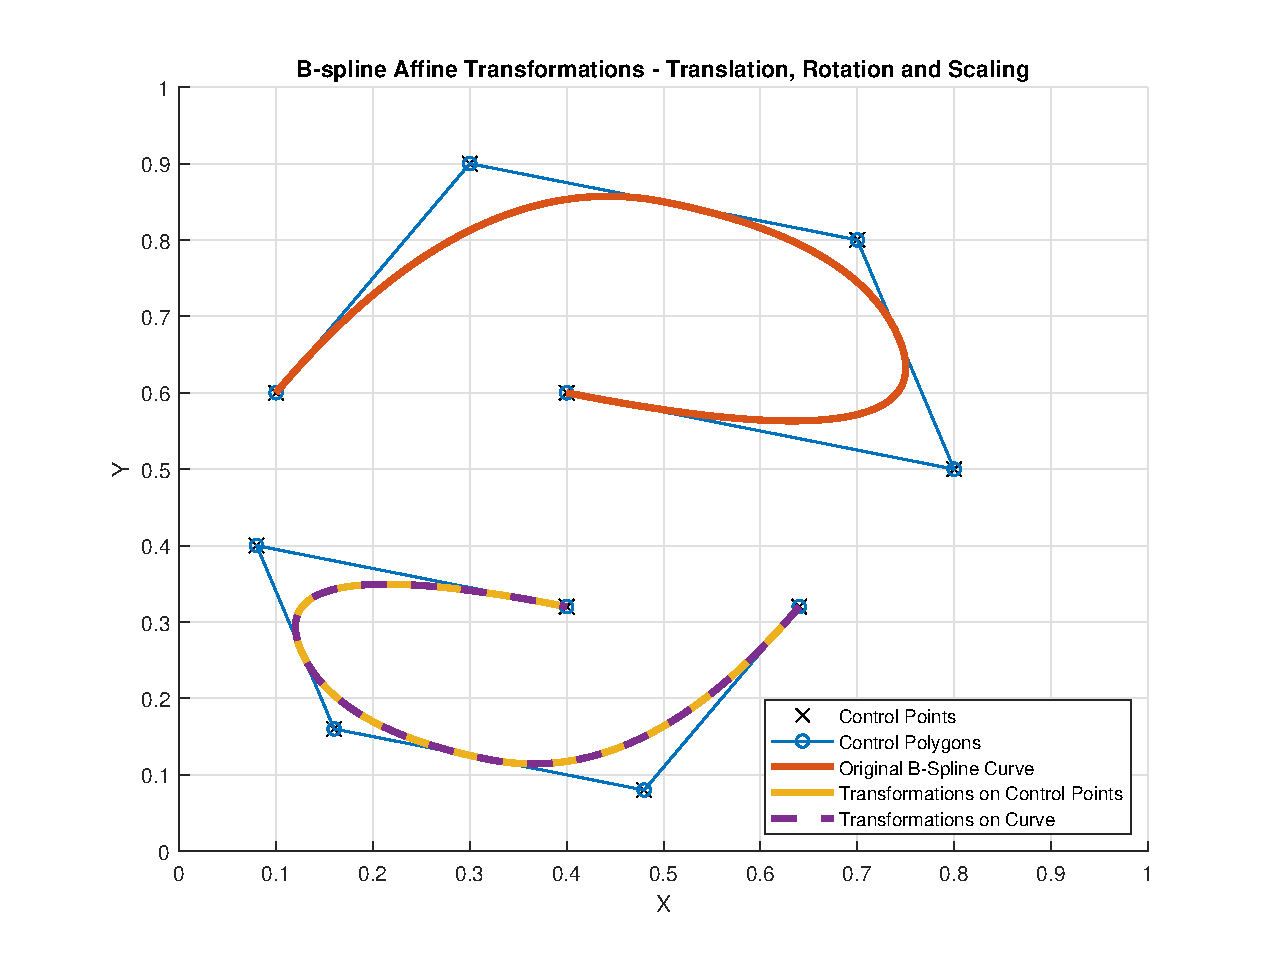
\includegraphics[scale=0.55]{plot_curve_affine_trans.eps}
	\label{fig:transAffCurve}
\end{figure}


\paragraph{Località.}
Muovendo $\mathbf{d_i}$ la curva $\mathbf{X}(t)$ cambia solo nell’intervallo $[t_i; t_{i+k})$. Questo segue dal fatto che $N_{i, k}(t) = 0$ per $t \notin [t_i; t_{i+k})$. Equivalentemente, $\mathbf{d_i}$ influenza solo al più $k$ segmenti di curva.

Negli script \ref{code:locality} e \ref{code:locality2} viene mostrata la proprietà di località. Nel primo script \ref{code:locality} viene mostrata come descritta sopra, ovvero data una B-Spline con $10$ punti di controllo, spostando il quinto punto la curva  varia solamente nell'intervallo $[t_5,t_9]$. Questo comportamento lo si può vedere in Figura \ref{fig:locality}. La proprietà di località ci dice anche che una curva B-Spline $\mathbf{X}(t^*)$ con $t^* \in [t_r,t_{r+1}]$ è determinata da $k$ punti di controllo $d_{e-k+1},\dots,d_r$. Nello script \ref{code:locality2} è mostrato questo comportamento, scegliendo $r=6$ e modificando i punti di controllo $d_j \notin [d_3, d_6]$ la curva $\mathbf{X}(t^*)$ rimane invariata per $t^* \in [t_6,t_7)$ come si può vedere in Figura \ref{fig:locality2}.

\lstinputlisting[label=code:locality, style=Matlab-editor, caption=Proprietà di Località, basicstyle=\footnotesize\ttfamily]{../b_spline_locality.m}

\lstinputlisting[label=code:locality2, style=Matlab-editor, caption=Proprietà di Località 2, basicstyle=\footnotesize\ttfamily]{../b_spline_locality_2.m}

\begin{figure}[h!]
	\centering
	\caption{B-spline Località}
	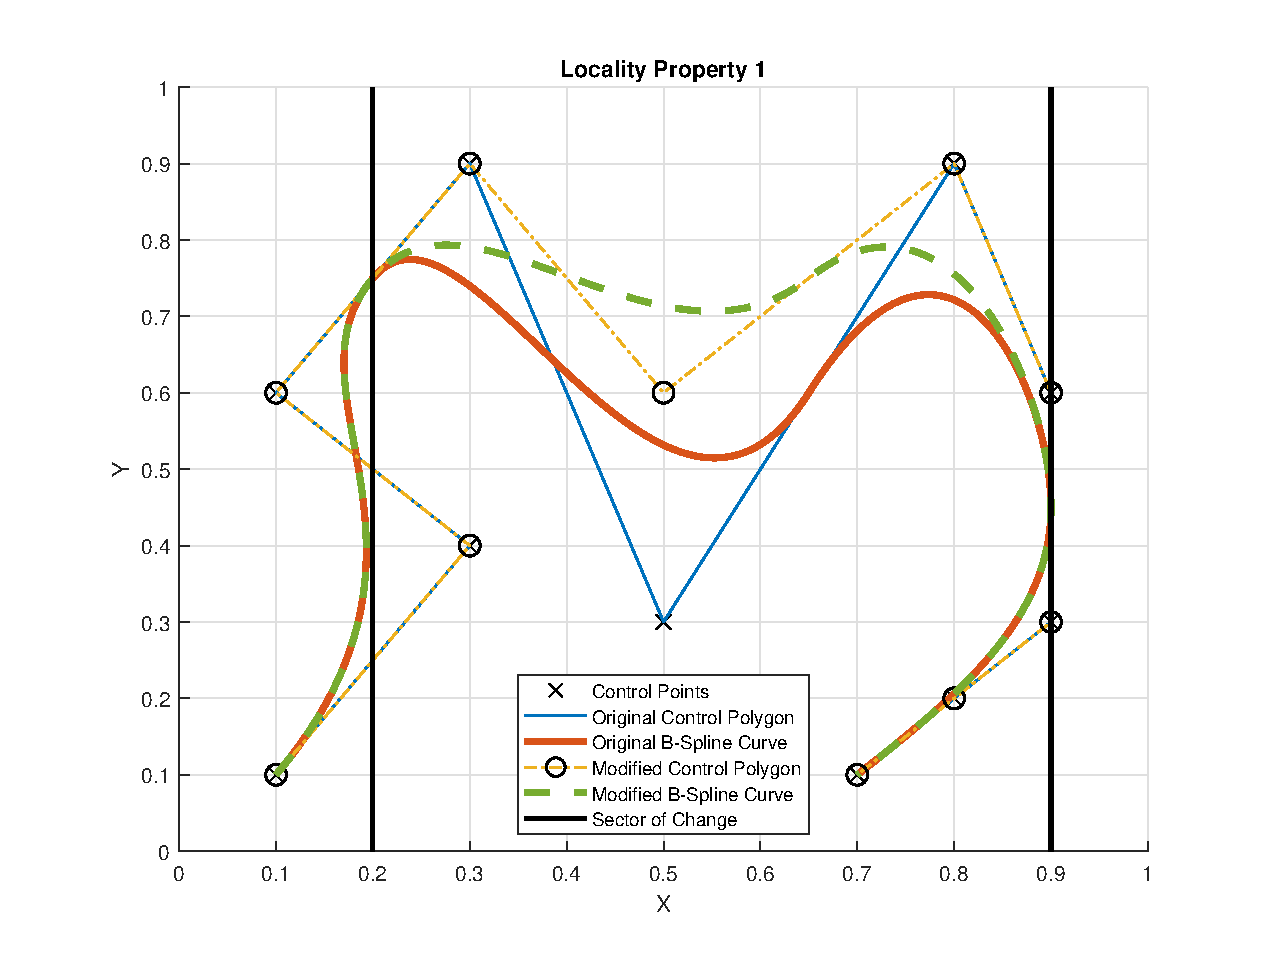
\includegraphics[scale=0.55]{plot_locality.eps}
	\label{fig:locality}
\end{figure}

\begin{figure}[!]
	\centering
	\caption{B-spline Località 2}
	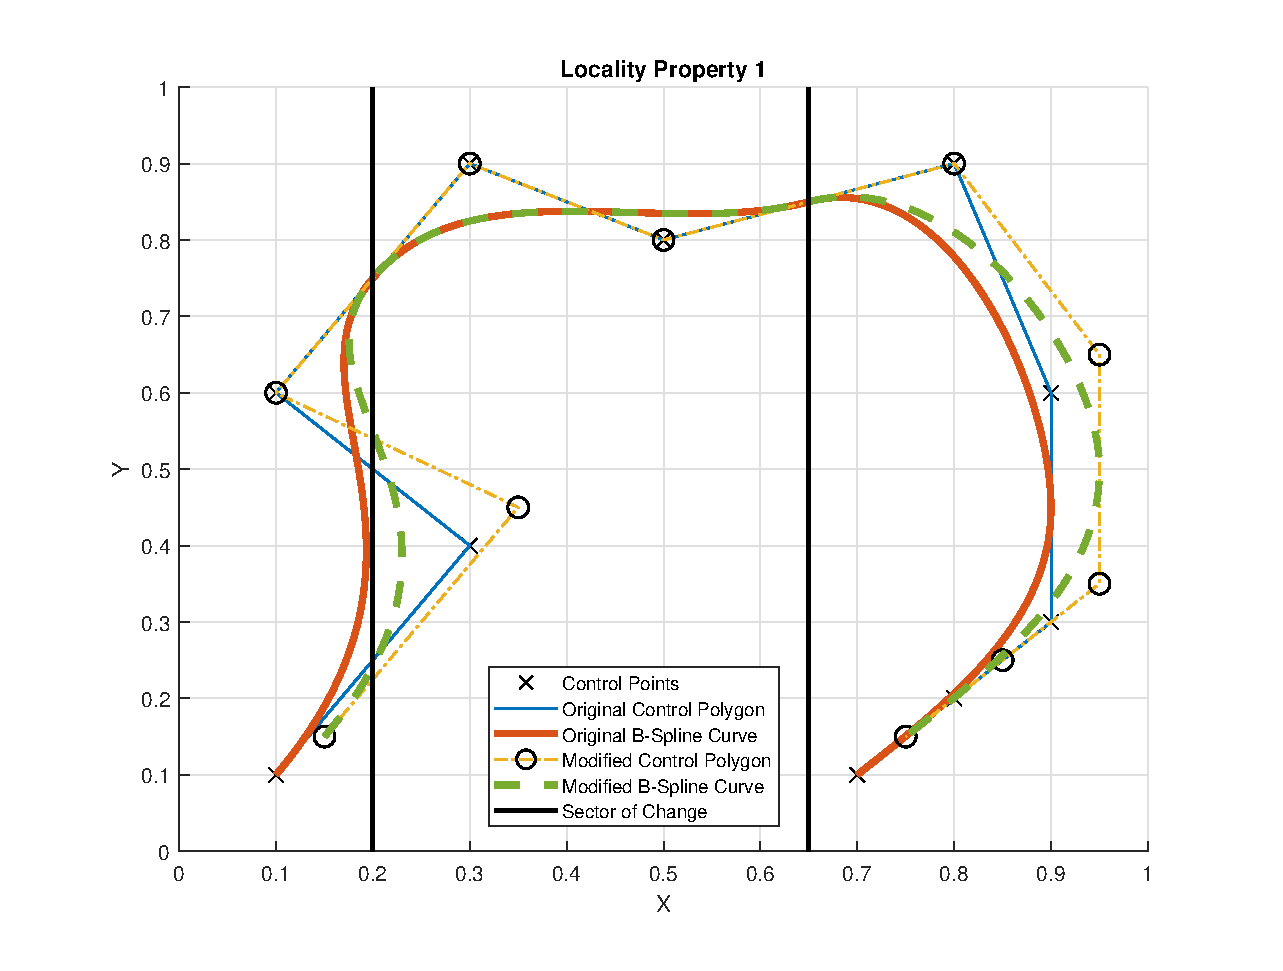
\includegraphics[scale=0.55]{plot_locality_2.eps}
	\label{fig:locality2}
\end{figure}

\paragraph{Strong Convex Hull.}
La curva è contenuta nel guscio convesso del suo poligono di controllo.

\paragraph{Variation Diminishing.}
Il numero di intersezioni tra la curva e una retta qualunque (un piano per le curve
nello spazio) è minore o uguale al numero di intersezioni tra il poligono di controllo e tale retta (piano). Ne segue che:
\begin{itemize}
	\item Se il poligono di controllo è convesso, la curva è convessa.
	\item Il numero di cambi di concavità della curva è minore o uguale al numero di
	      cambi di concavità del poligono di controllo.
\end{itemize}

Nello script \ref{code:BSplineCurveVariationDiminishing} è mostrata questa proprietà. Fissata una curva B-Spline, sono stati generati due punti randomici per i quali far passare una retta. Qualsiasi retta generata dallo script avrà un numero di intersezioni con la curva minore o uguale al numero di intersezioni con il poligono di controllo.\\
Nella figura \ref{fig:vardimcurve} sono raffigurati quattro esempi risultanti dall'esecuzione dello script \ref{code:BSplineCurveVariationDiminishing}.

\begin{figure}
	\begin{subfigure}{6cm}
		\centering 
		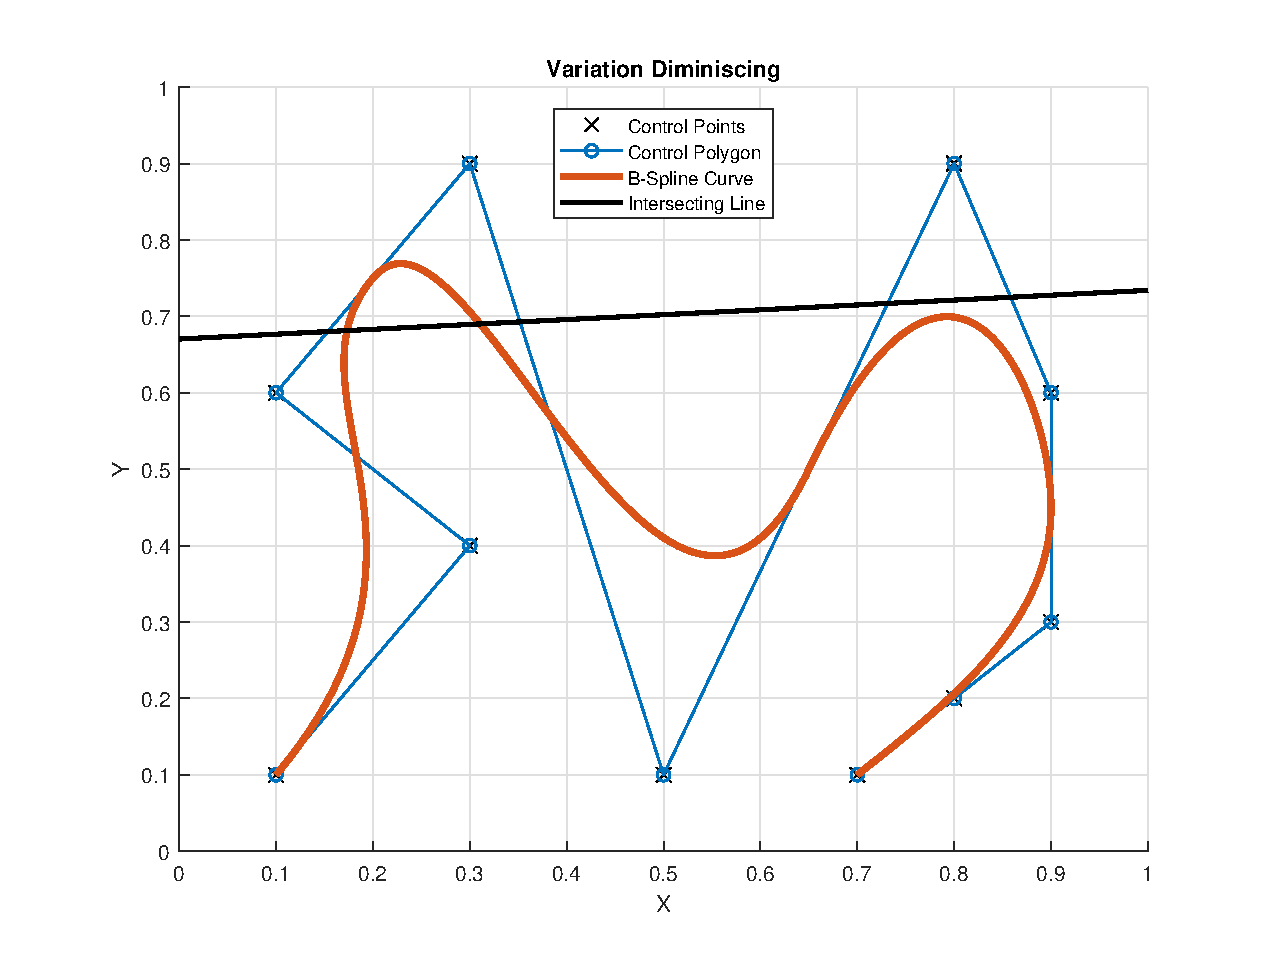
\includegraphics[width=6cm]{plot_variation_diminiscing_1.eps}
		%\caption{Caption text 1}
	\end{subfigure}
	\begin{subfigure}{6cm}
		\centering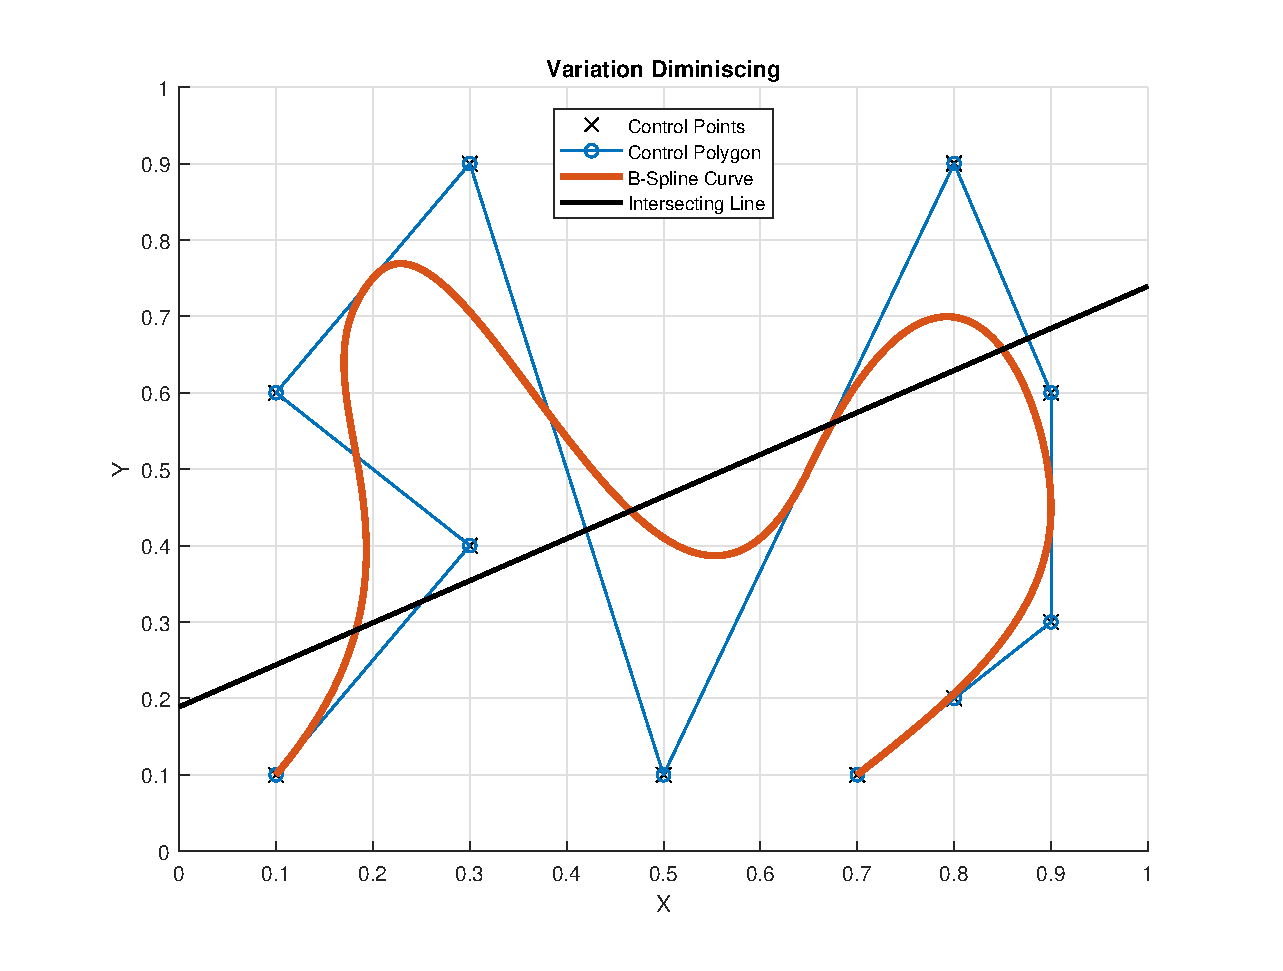
\includegraphics[width=6cm]{plot_variation_diminiscing_2.eps}
		%\caption{Caption text 2}
	\end{subfigure}
	
	\begin{subfigure}{6cm}
		\centering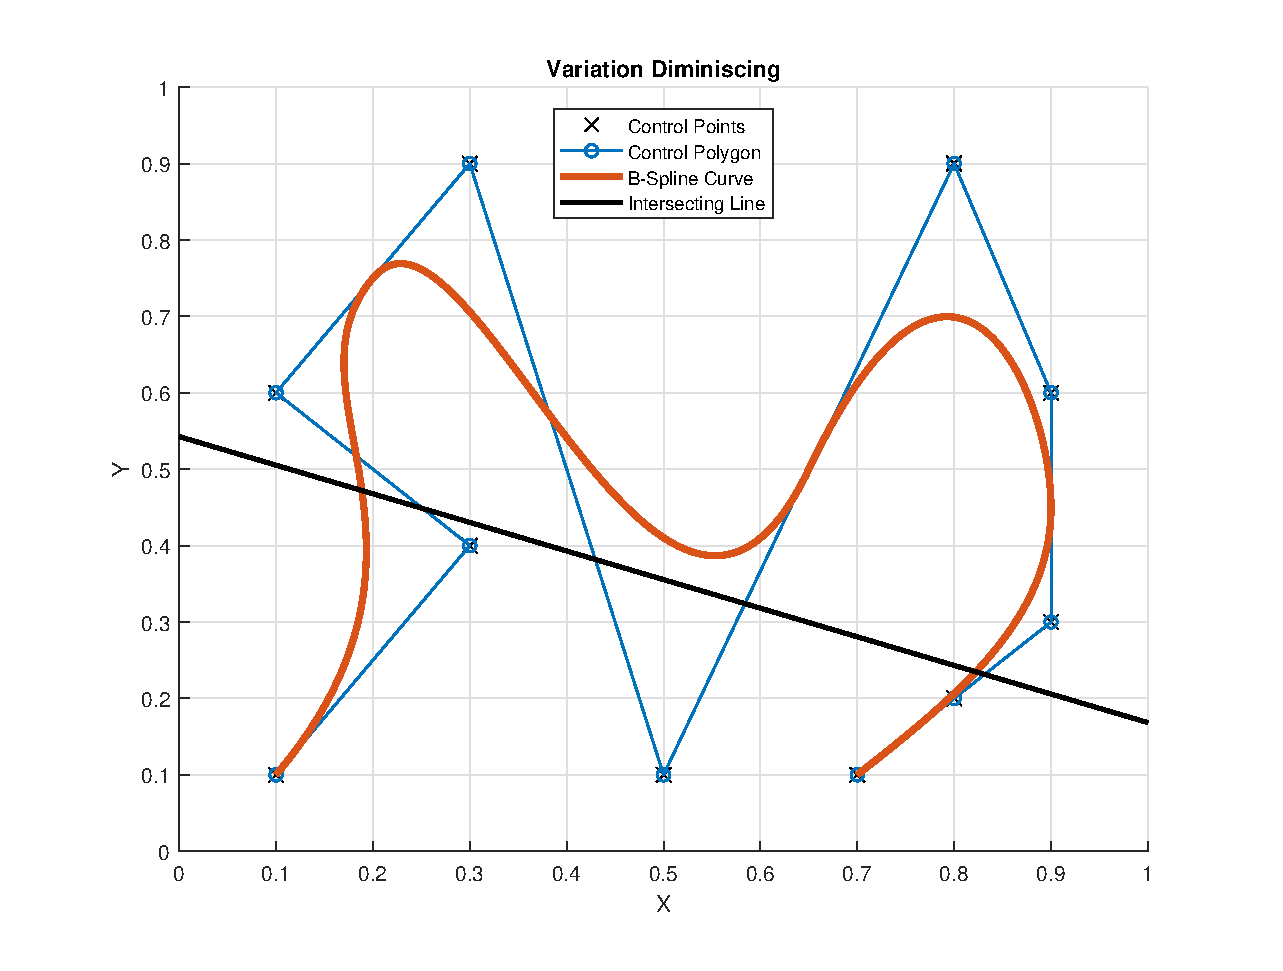
\includegraphics[width=6cm]{plot_variation_diminiscing_3.eps}
		%\caption{Caption text 3}
	\end{subfigure}
	\begin{subfigure}{6cm}
		\centering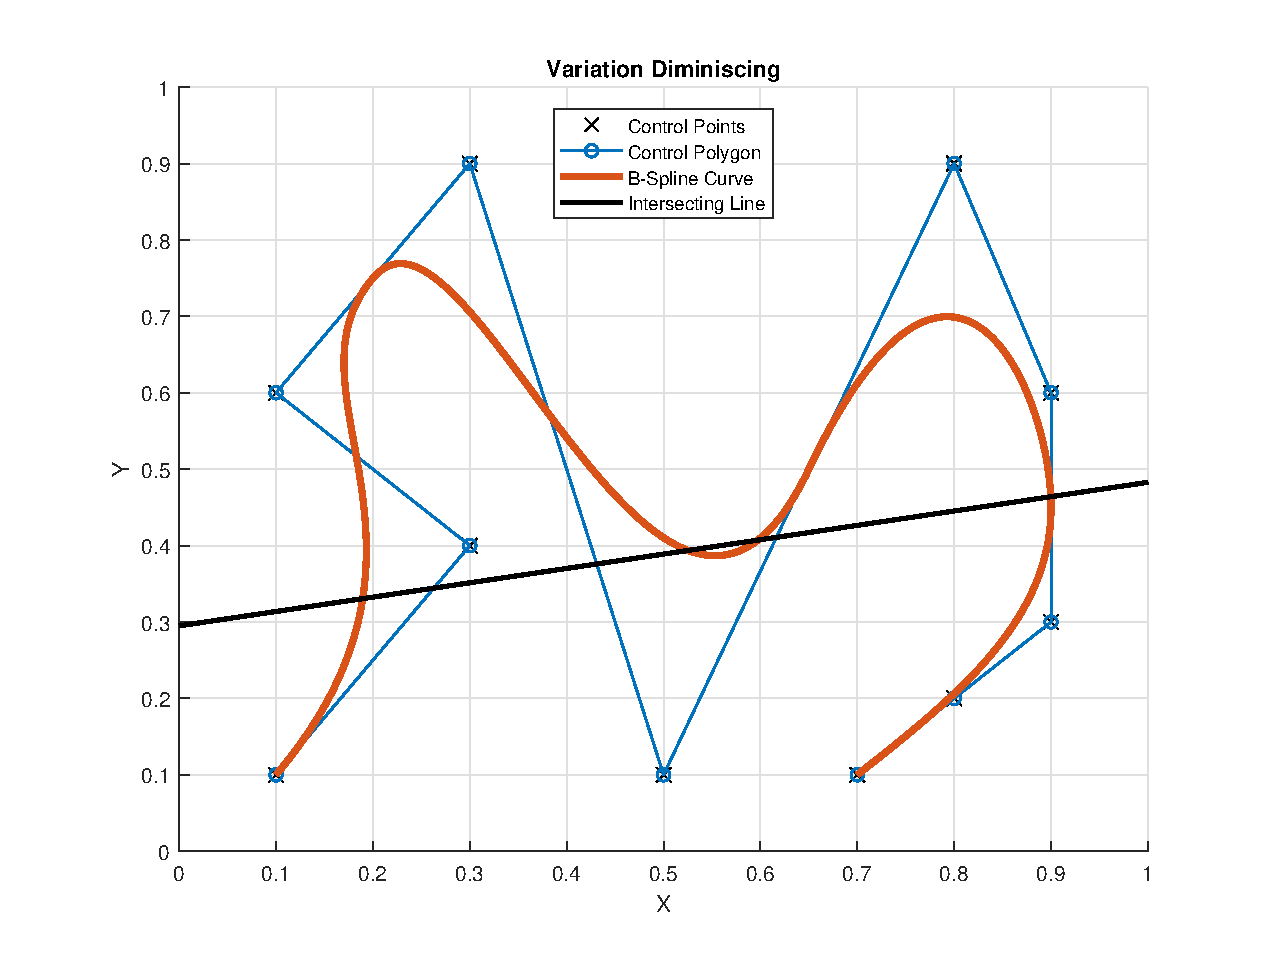
\includegraphics[width=6cm]{plot_variation_diminiscing_4.eps}
		%\caption{Caption text 4}
	\end{subfigure}
	\caption{Variation diminishing, quattro esempi di rette}
	\label{fig:vardimcurve}
\end{figure}


\lstinputlisting[label=code:BSplineCurveVariationDiminishing, style=Matlab-editor, caption=Variation diminishing, basicstyle=\footnotesize\ttfamily]{../b_spline_curve_variation_diminiscing.m}

\subsection{Rappresentazione di curve B-SPline chiuse}
Siano $\mathbf{d}_1,\dots \mathbf{d}_m$ i vertici di controllo del poligono chiuso (con $\mathbf{d}_1 = \mathbf{d}_m$). 
Per definire una curva B-SPline chiusa di ordine $k$, si sceglie la partizione nodale $$\mathbf{t} = \left[ \frac{-k}{m-1} : \frac{1}{m-1} : \frac{k+m-1}{m-1} \right]$$
e si estende il poligono di controllo  aggiungendo i vertici $$\mathbf{d}_{m+1} = \mathbf{d}_2,\mathbf{d}_{m+2} = \mathbf{d}_3, \dots, \mathbf{d}_{m+k-1} = \mathbf{d}_k, \mathbf{d}_{m+k} = \mathbf{d}_{k+1} $$

Lo script Matlab \ref{code:BSplineClosed}, dati in input il grado della curva ed i vertici di controllo, costruisce una curva B-Spline chiusa generando la partizione nodale estesa ed estendendo il poligono di controllo come descritto sopra. In figura \ref{fig:BSplineClosed} è riportato un esempio di curva B-Spline chiusa di ordine quattro con dieci vertici di controllo generata dallo script \ref{code:BSplineClosed} .

\lstinputlisting[label=code:BSplineClosed, style=Matlab-editor, caption=Curva B-Spline Chiusa, basicstyle=\footnotesize\ttfamily]{../b_spline_closed.m}

\begin{figure}[!]
	\centering
	\caption{Esempio di B-spline Chiusa}
	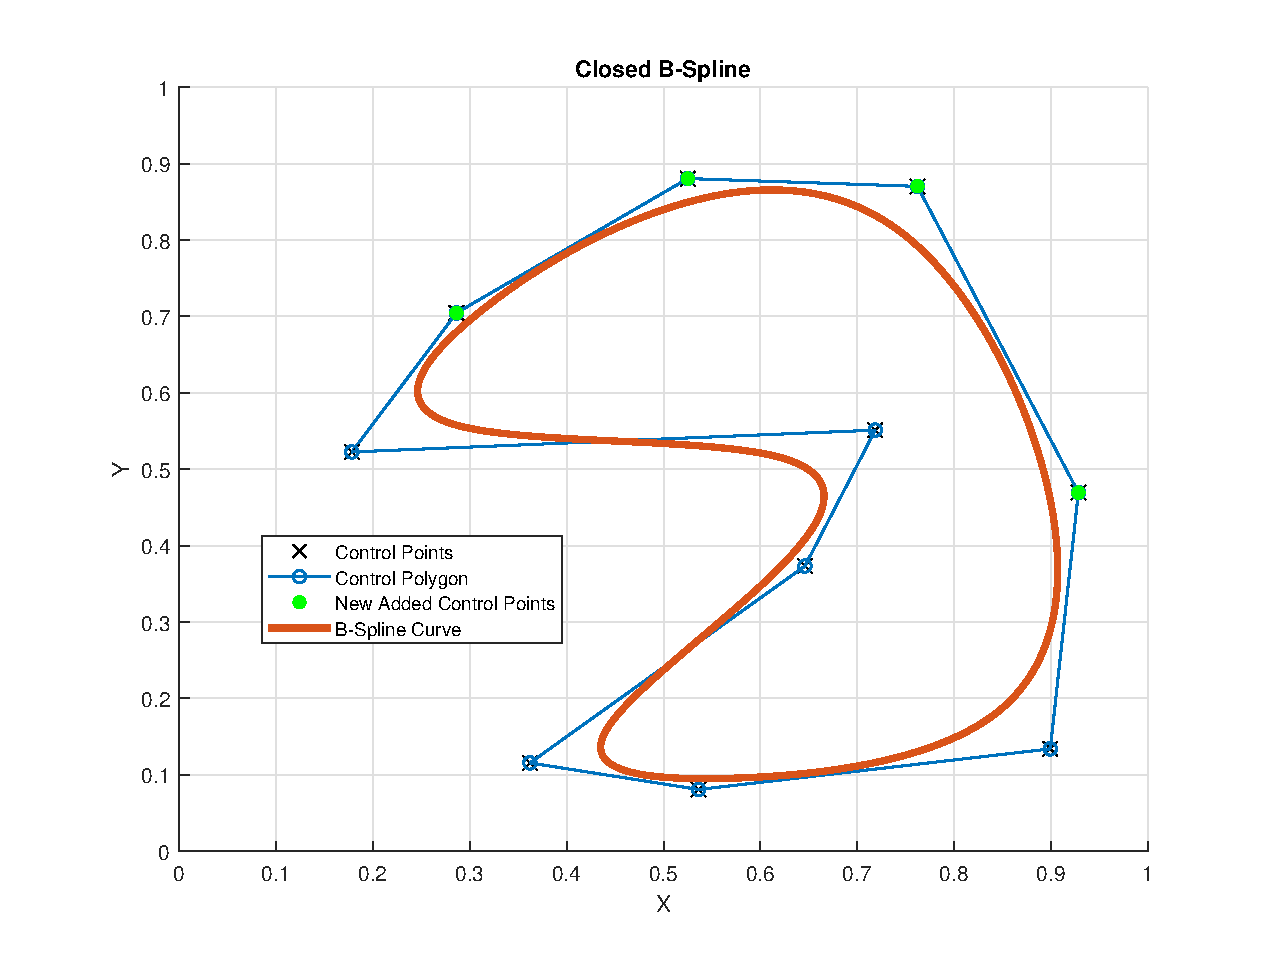
\includegraphics[scale=0.55]{plot_closed.eps}
	\label{fig:BSplineClosed}
\end{figure}

\end{document}          
